






\subsubsection{Le TOP500 et le benchmark HPL}

\paragraph{Le benchmarking ou l'étalonnage} est une pratique courante qui consiste à évaluer plusieurs solutions en leur faisant passer un épreuve commune. Dans le domaine informatique cela permet de tester différentes architectures matériels et d'évaluer laquelle sera la plus performantes. Il existe plusieurs benchmark qui ont chacune leur particularités. Ces codes essayent de reproduire les opérations faites par des codes industriels, dans le but de faire des projections de performances et pouvoir comparer deux solutions. Le benchmark le plus populaire dans le domaine du HPC est celui développé par Jack Dongara en 1988: le benchmark HPL \cite{Dongarra}. C'est grâce à lui que le classement du TOP500 est réalisé deux fois par ans.


\paragraph{Le TOP500} \footnote{\url{www.top500.org}} est un classement mondial qui classe, tous les 6 mois depuis 1993, les 500 super-calculateurs les plus puissants au monde. Ce classement se base sur le nombre maximum d'opérations flottantes qui peuvent être exécutées en une secondes. Cette unité à été choisie car la grande majorité des codes utilisés dans les domaines précédemment cités, exécutent des opérations sur des nombres flottant. Il s'avère donc judicieux de choisir ce dénominateur commun pour comparer les différentes architectures.  Une opération flottante peut être traduite par \textit{floating point operation} ou FLOP en anglais, on parlera donc de FLOP/S ou FLOPS pour désigner le nombre d'opérations flottante par seconde. Pour réaliser ce benchmark tous les supercalculteurs doivent exécuter le même code, le benchmark LINPACK \cite{Dongarra} \cite{450b1baca0774fd0976ff739b90bed04}. Ce benchmark est un code simple qui résout un système d'équation linéaire de deux matrices $A$ et $B$ par $Ax = B$. L'avantage de ce code est que les performances évoluent linéairement avec le nombre de machines utilisées car il y a très peu de communication sur le réseaux. Le résultat est un nombre de FLOP/S que la machine peut exécuter, ce qui rend la comparaison avec d'autres supercalculateur facile. 



Le site web du \textit{top500} contient de nombreuses données. On peut par exemple voir la consommation électrique, le nombre de coeurs, ou encore si les clusters contiennent des cartes graphique. Sur le graphique \ref{pic_top500perf_evo}, on voit que la puissances des supercalculateurs augmente d'un facteur 1000 tous les 10 ans.
Il faut cependant savoir que ce classement ne contient pas toutes les machines. En effet, certains industriels ne préfèrent pas paraître dans ce classement. Stratégiquement parlant, il peut être intéressant de ne pas publier sa puissance de calcul et nous savons que les clusters les plus puissants n'y figurent pas. Cependant ce classement nous permet de voir les tendances que suivent la majorité des architectures pour comprendre comment elles évoluent.\\

\begin{figure}
    \center
    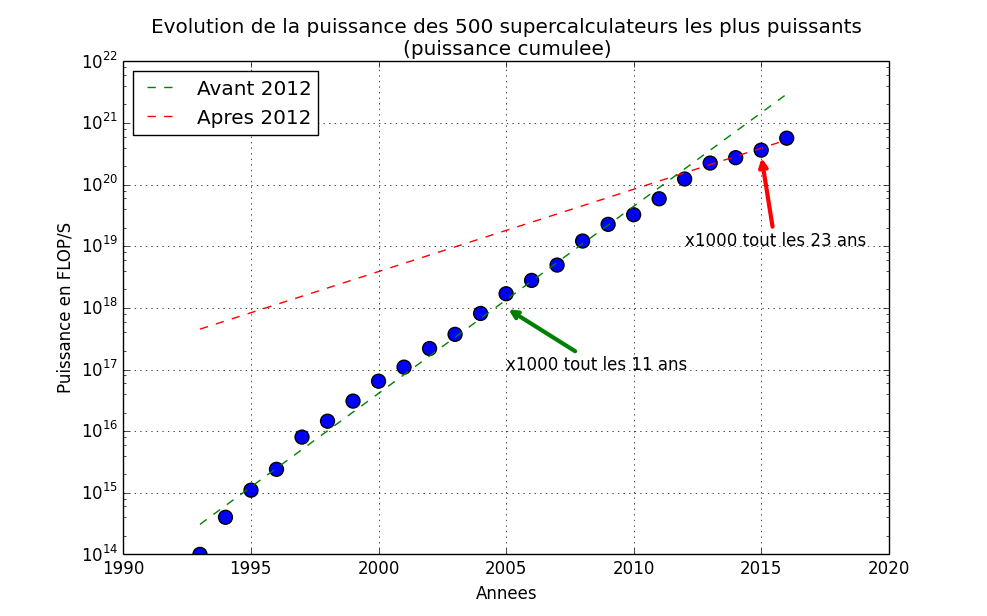
\includegraphics[width=10cm]{images/Chapitre1/pic_top500perf_evo.png}
    \caption{\label{pic_top500perf_evo} Évolution de la performance cumulée des 500 supercalculateurs les plus puissants au monde. La pente de l'évolution diminue à partir de 2012}
\end{figure}


Il existe un second classement qui classe les supercalculateur en fonction de leur ratio $\frac{FLOPS}{WATT}$ nommé le \textit{Green500} \cite{feng2007green500}. Comme nous allons le voir ensuite, la consommation électrique est devenus une contrainte forte dans l'architecture des nouveaux cluster. De plus en plus, la question n'est plus de construire le supercalculateur le plus puissant, mais le plus efficace.

\subsubsection{HPC ou HTC}
Aujourd'hui le domaine des supercalculateurs est souvent désigné par le terme HPC, mais il y a quelques précision à apporter quant à la mauvaise utilisation de ce terme. Il existe un autre domaine qui utilise les supercalculateur, le High Throughput Computing (HTC). En effet, la communauté à voulu donner un nom aux architectures capables d'exécuter différentes applications simultanément et ce sans interruptions sur plusieurs mois. Contrairement aux applications HPC qui exécutent des taches très dépendantes les unes des autres, les applications HTC se focalisent sur l'exécution des plusieurs tâches en parallèles et assure la disponibilité maximale du nombre de ressources dont dispose le supercalculateur. Prenons pour exemple un cluster de calcul partagé dans une université. L'objectif de cette machine n'est pas d'exécuter une application toute l'année, mais plutôt de répartir le matériel disponible entre les utilisateurs pour que tous puissent l'utiliser au maximum. Une majorité des clusters d'aujourd'hui fonctionnent sur le même modèle et l'utilisation de l'expression HPC pour les désigner est en fait un abus de langage.




Alors que nous n'avons jamais eu besoin d'aussi grandes puissances de calcul, le graphique montre bien qu'il y a eu une inflexion en 2012. Le challenge principal inhérent au HPC est celui du cout des machines et donc celui du ratio $\frac{Prix}{FLOPS}$. Un autre challenge qui est apparu est celui de la puissance électrique nécessaire pour aliment les supercalculateurs. Les lignes électrique arrivant sur les sites, ne sont plus assez puissante pour que l'on puisse suivre la stratégie employée jusqu'à aujourd'hui qui était d'augmenter le nombre de machines pour augmenter la puissance de calcul. Aujourd'hui nous cherchons donc aussi à augmenter le ratio $\frac{Watt}{FLOPS}$ même si cette solution ne sera pas éternellement viable comme l'a prédit \cite{5392446}.
Enfin, les clients du HPC acquièrent plus de données que jamais et les clusters doivent pouvoir les contenir et les traiter dans des délais raisonnable. En effet les objets connectés qui génèrent de gigantesques quantité de données doivent être capables d'en traiter une partie sur place avec des moyens souvent limité (énergie, puissance de calculs). Ces challenges sont donc applicables au data center mais aussi à l'extérieur si nous voulons être capable de prendre des décisions en temps réel, comme pour les voitures autonomes qui n'auront que quelques micro secondes pour réagir en cas d'accident. Le travail présenté dans cette thèse est donc nécessaire pour pouvoir accéder à toutes ces promesses que nous réserve l'avenir.


\subsubsection{Systèmes non-équilibrés}

La précision des simulations, les approches multi-physique ainsi que les objets connectés produisent des volumes de données à gérer et à analyser tels qu'ils ont été caractérisé par la communauté de déluge %\cite{bodin:hal-01174302}.
En conséquence, l'exploitation et la gestion des données sont l'autre pan de l'évolution des logicielles qui va bouleverser les pratiques. Une majorité des applications HPC autrefois centrée sur une problématique de puissance de calcul sont maintenant fortement limitées par le traitement des données pour deux raisons: une augmentation très forte de la puissance des processeurs contre une faible augmentation de la quantité de données que les mémoires peuvent leur délivrer. Si on regarde l'évolution des performances des différentes parties du système on peut constater de réelles différences:
\begin{itemize}
    \item Les performances calculatoirs des processeurs (le nombre d'opération flotantes réalisables par cycle) à \textbf{augmenté de 50\%} en moyenne par an.
    \item La bande passante entre le processeur et la mémoire à augmenté de 23\% par an
    \item La lantence des requêtes mémoire a \textbf{augmenté de 4\% }par an
    \item La bande passante sur le réseau à \textbf{augmenté de 20\%} par an
\end{itemize}

\begin{figure}
    \center
    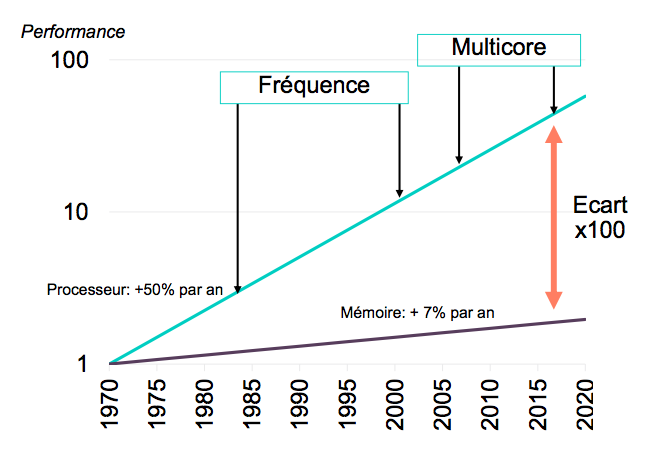
\includegraphics[width=10cm]{images/Chapitre1/memory_gap.png}
    \caption{\label{pic_memory_gap} Différence de l'évolution des performances des processeurs et des mémoires }
\end{figure}

On voit donc que la puissance des processeurs à augmenté bien plus rapidement que celle des mémoires. Les processeurs ont béféniciés de nombreuse amélioration. L'augmentation de la fréquences par exemple, ou le nombre de coeurs par processeur. Ainsi les performances des systèmes ne sont plus équilibrées et les architectures ont du s'adapter notamment avec l'apparition d'une hierarchie mémoire, plus au moins rapide et plus ou moins grande. L'apparition des caches à permis d'augmenter la performance relative des applications en camouflant l'augmentation faible de la bande passante. Cela à contribué à l'augmentation de la complexité des architectures et il faut désormais au programmeur des connaissances solides pour aller tirer le maximum de performances de ces processeurs

\textbf{TODO: annoncer le plan de these}